A \textit{convolução} é uma operação linear que calcula a soma dos produtos de toda a extensão de duas entradas em função de um determinado deslocamento. Essa operação é a propriedade fundamental da camada convolucional, a principal camada de uma CNN \cite{ref:goodfellow}.  O principal objetivo da operação de convolução nas CNN é a extração das características de uma determinada entrada \cite{ref:sewak}. 

O processo de convolução utilizado nas CNNs é aplicado em um conjunto de \textit{filtros} e uma dada entrada para gerar uma saída conhecida como \textit{mapa de características}. A camada convolucional recebe um volume de entrada de $n$ dimensões e pode possuir um preenchimento  $p$ de zeros (\textit{zero-padding}), aplicado ao redor da entrada. Essa entrada é processada por $k$ filtros que representam os pesos e as conexões da CNN \cite{ref:khan}. Cada filtro consiste em uma matriz de números discretos e possui uma extensão espacial $e$, que é igual ao valor da altura e da largura do filtro, e um \textit{stride} $s$, que é a distância entre as aplicações de convolução consecutivas do filtro no volume de entrada \cite{ref:buduma}. 

A Figura \ref{img:convolucao} exemplifica o processo de convolução aplicado em uma entrada de tamanho 5 x 5 e \textit{zero-padding} $p = 1$. O filtro utilizado no exemplo possui extensão espacial $e = 2$ e \textit{stride} $s = 2$ com inicialização de pesos aleatória. É possível observar que o mapa de características é uma saída de tamanho 3 x 3 em que cada um dos seus componentes é a da soma das multiplicações dos elementos do filtro com os elementos de um segmento da entrada \cite{ref:khan}.

\begin{figure}[!ht]
	\centering
	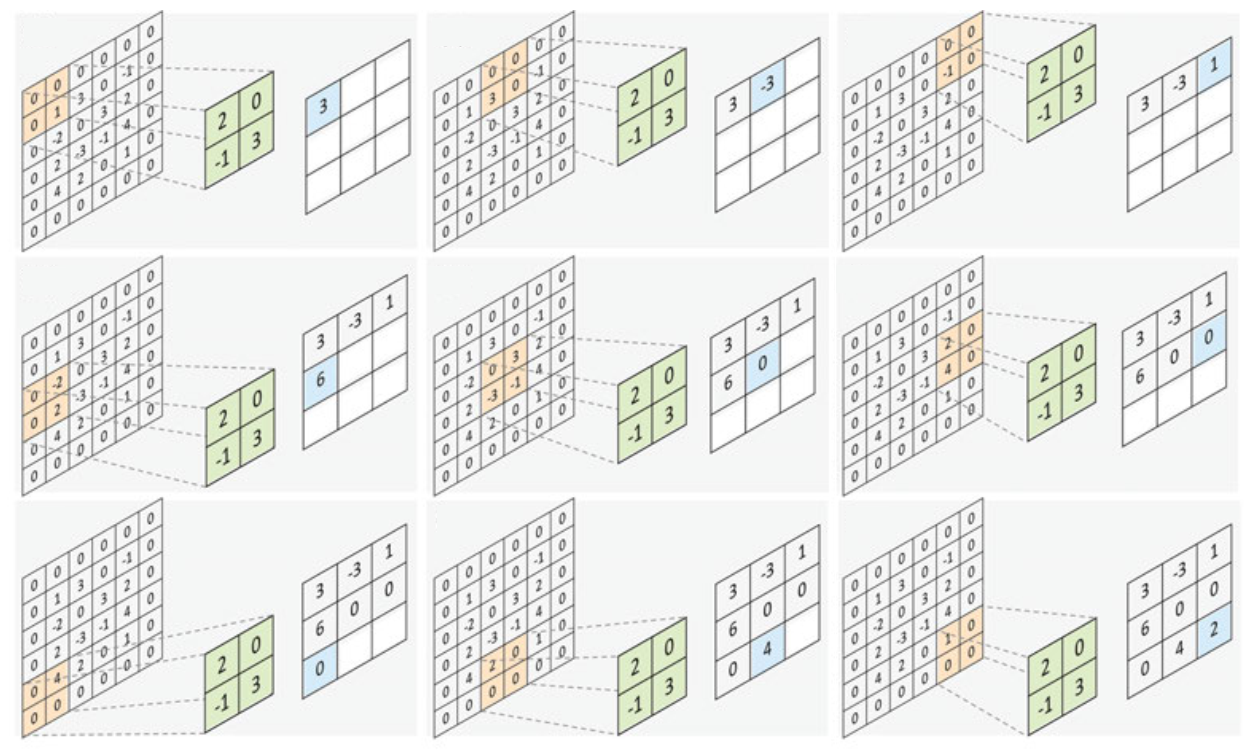
\includegraphics[width=0.9\textwidth]{./img/convolucao}
	\caption{Exemplo de um processo de convolução aplicado em uma entrada de tamanho 5 x 5 e um filtro de tamanho 2 x 2. Fonte: \cite{ref:khan}.}
	\label{img:convolucao}
\end{figure}


